\chapter{緒論}
\label{c:introduction}

以下文中的$\backslash$皆代表latex中輸入指令的前綴,因直接打反斜線會編譯不過~~。

\section{封面}
\label{sec:cover}

封面的設定在nthuvars.tex與nthuthesis.cls中,前者是輸入封面頁上的各式文字(標題、姓名等等),後者則是管理封面的樣式,格式若要更改請自行修改nthuthesis.cls的60-88行。

若用於proposal則將66行註解、67行清除註解,用於碩士論文就是66行清除註解67行註解這樣。

\section{文章架構}
\label{sec:architecture}

論文由大至小依序為章、節、小節以及標題列舉,章、節請參考上面的定義,其餘設置如下:

\subsection{我是小節}
\label{subsec:subsection}

\subsubsection{我是標題列舉}
\label{subsubsec:subsubsection}

其中包含標題名稱與label,前者是文中顯示的樣子,後者是要引用時所需要的標籤,因此後者可以修改成你喜歡的格式都可以,方便用就好,如果沒有要引用也可以不加。

在寫作時由於文章會很長,因此可以切割成多個.tex檔案,筆者是以chapter為單位切開,新增檔案記得要去thesis.tex中input進去(參考thesis.tex中173-174、179-204行)。

\section{圖片}
\label{sec:fig}

所有的圖片都存在figsrc資料夾內,因為圖片很多所以可以自行新增子資料夾在內,那以筆者緒論中的圖片為例,首先是單張圖片,分成svg與非svg,svg檔有時候會編譯不過(似乎只是beta版),因此筆者後來就將svg幾乎全部轉為PDF使用,插入svg使用$\backslash$includesvg{}[],其餘常見圖片格式應該都可以用$\backslash$includegraphics{}[],中括號內可指定圖片尺寸,常見都是根據紙張扣除邊界的大小進行比例設定,如[width=0.8 $\backslash$textwidth]。或是可以跟筆者一樣,畫圖時直接畫好指定大小,載入時直接以原尺寸載入即可(如\cref{fig:mrs_framework})。

\begin{figure}[htbp]
    \centering
    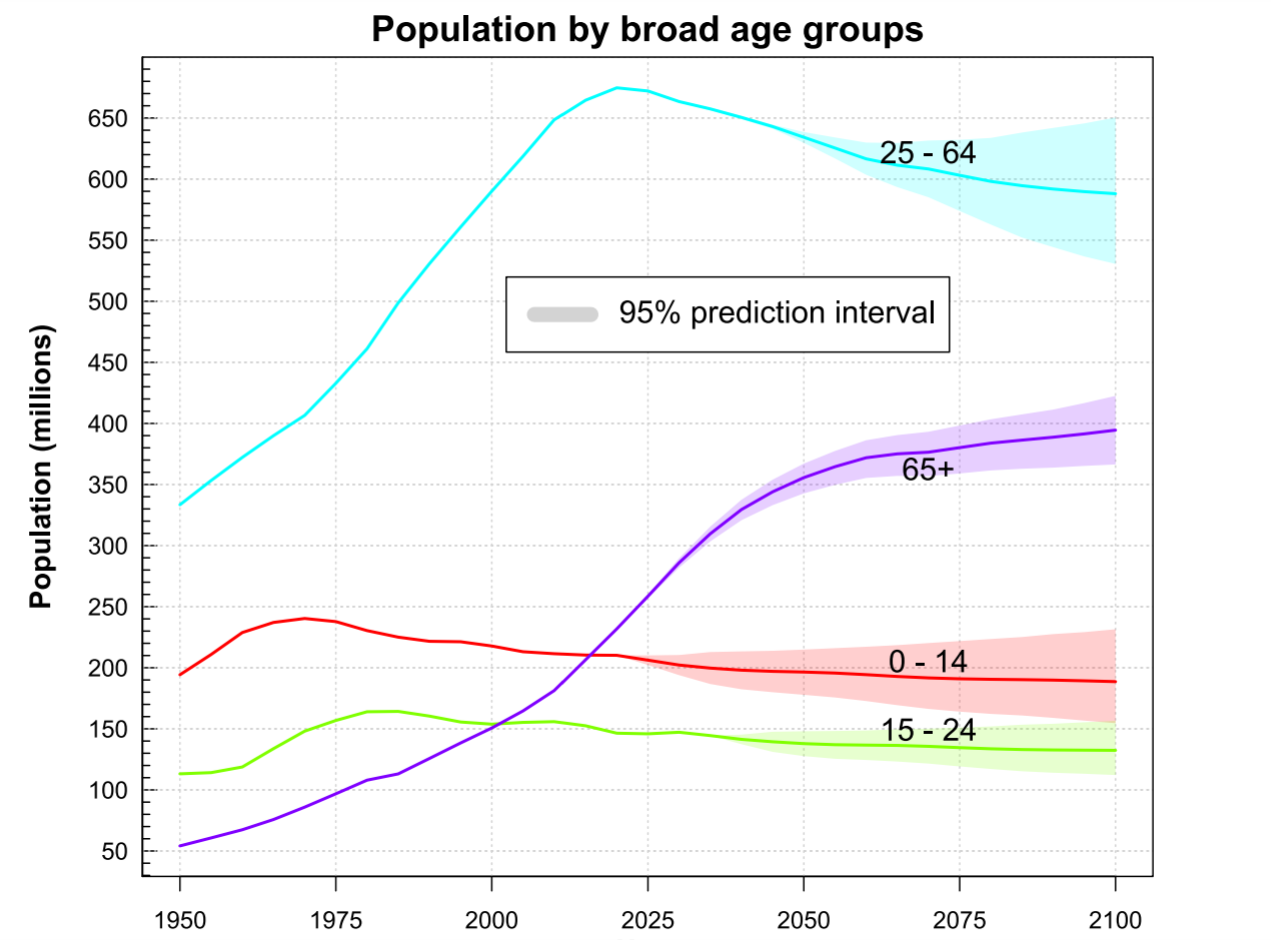
\includegraphics[width=0.8\textwidth]{figsrc/ch01/high_income_population_by_age_groups.png}
    \caption{高收入國家之年齡組別人口成長預測圖\cite{nations2019world}}
    \label{fig:population_age_world}
\end{figure}

\begin{figure}[htbp]
    \centering
    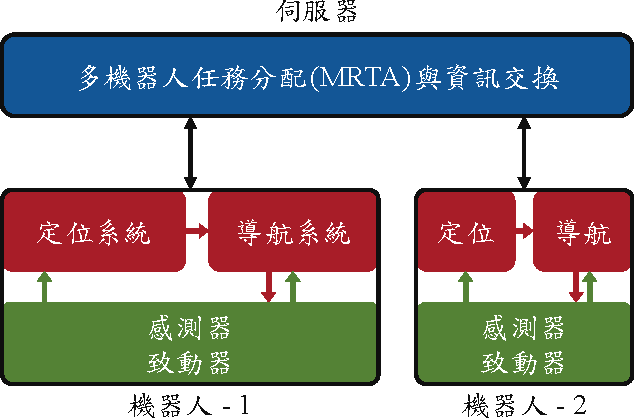
\includegraphics{figsrc/ch01/mrs_framework_zh.pdf}
    \caption{多機器人系統架構圖}
    \label{fig:mrs_framework}
\end{figure}

\begin{figure}[htbp]
    \centering
    \includesvg[width=0.9\textwidth]{figsrc/ch01/taiwan_population.svg}
    \caption{三階段年齡人口變動趨勢\cite{國發會年齡人口變動趨勢}}
    \label{fig:population_age_taiwan}
\end{figure}

有時候需要將圖片並排,可以參考以下的說明,其中建立兩個subfigure,其總大小需要稍微比頁面寬度略小不然會超出去(若真的要超出去可以參考下方註解,但盡量不要,會破壞排版,也可以將整個圖/表轉90度,參考\cref{c:appendix_caption}),故這邊設定單個子圖為0.48倍的頁面寬度,讓兩張圖一樣寬,有需要的話也可以自行調整兩者比例,$\backslash$hfill的目的是在兩張圖中間填充需要的空白,如果你的圖真的塞得有點極限也可以拿掉看看會不會就塞得進去。另外圖名(或是所有用到caption的地方),$\backslash$caption[顯示於目錄的標題]{顯示於內文的標題}可自由使用,若有些資訊或是備註不想讓他在目錄出現,可以弄一個比較簡短的。

\begin{figure}[htbp]
    \centering
    \begin{subfigure}[b]{0.48\textwidth}
        \centering
        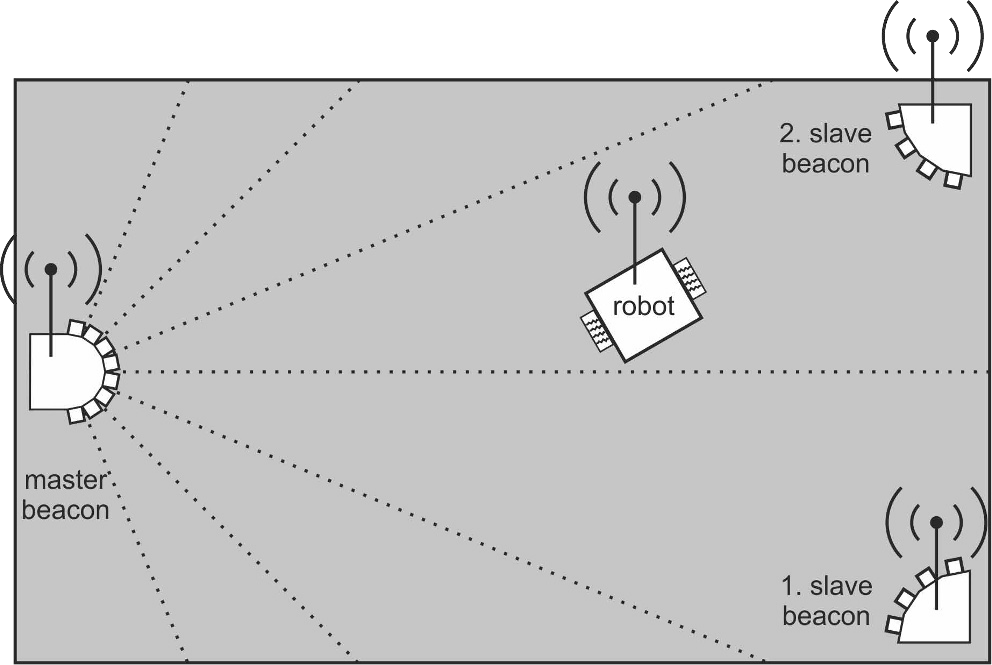
\includegraphics[width=\textwidth]{figsrc/ch01/eurobot_2012_ultrasonic_300dpi.png}
        \caption{超聲波定位系統示意圖\cite{eurobot_ultrasound_2013}}
        \label{fig:eurobot_2013_ultrasound}
    \end{subfigure}
    \hfill
    \begin{subfigure}[b]{0.48\textwidth}
        \centering
        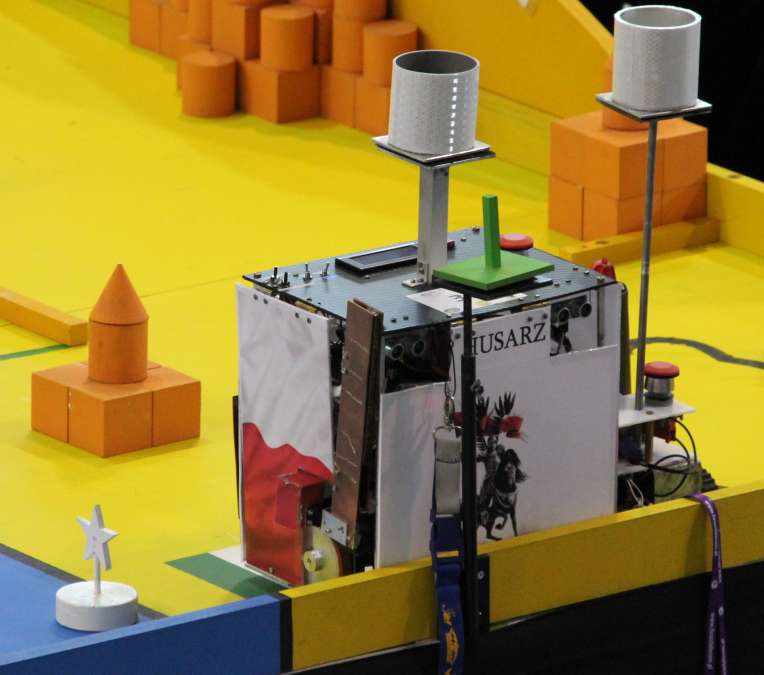
\includegraphics[width=\textwidth]{figsrc/ch01/eurobot_ros_2016_300dpi.png}
        \caption{SKaNeR所製作的機器人\cite{eurobot_ros_2016}}
        \label{fig:eurobot_ros_2016}
    \end{subfigure}
    \caption[隊伍於比賽時使用之系統示意圖與比賽實景(顯示於目錄的標題)]{隊伍於比賽時使用之系統示意圖與比賽實景(顯示於內文的標題)}
    \label{fig:eurobot_2013_2016}
\end{figure}

% 真的塞不下可考慮此方法,但需要依照情況微調
% \begin{figure}[htbp]
%     % figure is too large -> \centerline
%     \centerline{
%         \includegraphics[width=1.15\textwidth]{figsrc/ch04/sim_movement/eurobot_2022_0y1p_2.pdf}
%     }
%     \caption[模擬一:困難-2場景中三個演算法的導航結果]{模擬一:困難-2場景中三個演算法的導航結果(由左至右分別為APF、TEB及DWA的導航結果)}
%     \label{fig:sim_1_hard_2_movement}
% \end{figure}

\section{表格}
\label{sec:table}

表格通常會借助線上表格工具產生latex code後再貼入,筆者是使用\url{https://www.tablesgenerator.com/latex_tables}編輯後貼入,範例如\cref{table:exp_size}所示,而若需要整頁的表格請參考\cref{table:sim_1_result_sr_subopt_ta}。

\begin{table}[htbp]
\caption{實驗場域規格}
\label{table:exp_size}
\setlength{\tabcolsep}{7mm}
\begin{tabular}{lccc}
\hline
                           &    & 模擬環境  & 實驗環境  \\ \hline
\multirow{2}{*}{場地尺寸}      & 長  & 3m    & 4m    \\
                           & 寬  & 2m    & 2.3m  \\ \hline
\multirow{3}{*}{車輛尺寸}      & 長  & 0.2m  & 0.4m  \\
                           & 寬  & 0.2m  & 0.4m  \\
                           & 高  & 0.4m  & 0.3m  \\ \hline
\multirow{2}{*}{Beacon 尺寸} & 半徑 & 0.05m & 0.08m \\
                           & 高  & 0.51m & 0.29m \\ \hline
\end{tabular}
\end{table}

\section{方程式}
\label{sec:equation}

Latex語法用於打方程式應該是大家最熟悉的了,一樣有許多線上工具可以讓你打得更快,筆者這邊是使用\url{https://latex.codecogs.com/eqneditor/editor.php}協助產生一些少用的指令。也可以參考overleaf的官方文件:\url{https://www.overleaf.com/learn/latex/Mathematical_expressions},裡面有詳細說明這邊就不贅述,最簡單的就是用$a+b=c$這樣,以下是節錄自筆者論文內的方程式,使用align並且在thesis.tex中有設定可讓多個方程式跨頁方便排版。額外補充,\url{https://hackmd.io/@CynthiaChuang/Basic-LaTeX-Commands}這裡有人整理了常用數學符號指令。

\begin{align}
    \label{eqn:predict_mu_tf_zero}
	f(\boldsymbol{u}_{t},\boldsymbol{x}_{t}) &=
    \begin{bmatrix}
        v_{t}cos\theta\triangle t\\ 
        v_{t}sin\theta\triangle t\\ 
        0    \end{bmatrix}\\
    \label{eqn:predict_G_mat_zero}
    \boldsymbol{G}_t &= \begin{bmatrix}
    1 & 0 & -v_{t}sin\theta\triangle t\\
    0 & 1 & -v_{t}cos\theta\triangle t\\
    0 & 0 & 1 \end{bmatrix}\\
    \label{eqn:predict_V_mat_zero}
    \boldsymbol{V}_t &= \begin{bmatrix}
    cos\theta\triangle t & 0 \\    
    sin\theta\triangle t & 0 \\
    0 & 0 \end{bmatrix}\\
    \label{eqn:motion_noise_zero}
    \boldsymbol{M}_t &= \begin{bmatrix}
    \alpha_1 v_t^2 + \alpha_2\omega_t^2 & 0\\
    0 & \alpha_3 v_t^2 + \alpha_4\omega_t^2\\
    \end{bmatrix}
\end{align}

\section{演算法}
\label{sec:algorithm}

演算法也是有百百種用法,這邊使用的如下方所示,在thesis.tex 38行引用algorithm2e package,其餘請自行舉一反三XD。值得留意的是,有些老師會要求只有變數才能是斜體,若在演算法中要打方程式,要留意正體與斜體之間的差異,可以不要寫在方程式內(如下方calculate及return),或是使用$\backslash$text{}將文字括起來。

\begin{algorithm}[htbp]
\caption{EKF Localization: Predict Step}
\label{algo:ekf_predict}
\KwIn{$\boldsymbol{\mu}_{t-1}, \boldsymbol{\Sigma}_{t-1}, \boldsymbol{u}_{t}$}
\KwOut{$\boldsymbol{\bar{\mu}}_t, \boldsymbol{\bar{\Sigma}}_t$}
\BlankLine
calculate $f(\boldsymbol{u}_{t},\boldsymbol{x}_{t}), \boldsymbol{G}_t, \boldsymbol{V}_t, \boldsymbol{M}_t$\;
$\boldsymbol{\bar{\mu}}_t = \boldsymbol{\mu}_{t-1} + f(\boldsymbol{u}_{t},\boldsymbol{x}_{t})$\;
$\boldsymbol{\bar{\Sigma}}_t = \boldsymbol{G}_t \boldsymbol{\Sigma}_{t-1} \boldsymbol{G}_t^T + \boldsymbol{V}_t \boldsymbol{M}_t \boldsymbol{V}_t^T$\;
return $\boldsymbol{\bar{\mu}}_t, \boldsymbol{\bar{\Sigma}}_t$
\end{algorithm}

\section{列舉}
\label{sec:enumerate}

有時候會需要列舉的功能,原先的列舉每個標號之間空白太多,因此加上了[nosep],指令如下:

\begin{enumerate}[nosep]
\item 第一點
\item 第二點
\item 第三點
\end{enumerate}

\section{引用}
\label{sec:reference}

\subsection{文獻引用}

引用部分使用的是cite package,相關設定在thesis.tex 209-215行,目前設定為IEEEtran\_rchen的樣式,也就是依照動機系ICMEMS實驗室的論文模板魔改出來的特殊格式,若其他實驗室想使用此模板,建議將thesis.tex 210行改為IEEEtran格式並刪除暫存檔後重新編譯。所有文獻皆以BibLaTeX格式記錄在thesis.bib中(目前裡面是筆者的引用資料,提供給大家參考),可以使用google學術搜尋找到想引用的論文後,按cite找到他的BibLaTeX格式並複製貼上到thesis.bib中。

若是ICMEMS的實驗室同學請特別留意:
\begin{enumerate}[nosep]
\item @inproceedings(研討會論文),老師要求要有舉辦地點與詳細時間,因此可參考thesis.bib中的寫法補上address,範例如下:address={Bangkok, Thailand, December 14 - 17}。
\item @online(線上資料),此格式如\cite{eurobot}所示,請自行參閱thesis.bib中內容。
\item @emptymisc(空白的格式),若喬不好格式可用這個,完全自己打的reference,尤其是當要引用中文文獻時,避免全/半形標點符號混用,範例請見thesis.bib。
\end{enumerate}


以下範例擷取自筆者碩士論文中緒論的第一節:

隨著電子商務的蓬勃發展,物流與配送需求逐年上升。如在工廠內的揀貨,基本為勞力較為密集的產業。而隨著勞力成本提高,且業者越來越不容易找到願意從事此類單調生產工作的勞動人力,因此,應用於物流配送之自動化技術已成為顯學,如此不只能減緩缺工問題,也能提升貨品搬運效率、運送穩定度以及降低生產成本。

此外,根據聯合國經濟和社會事務部在2019年發布世界人口展望報告(World Population Prospects 2019)\cite{nations2019world}指出,儘管全球人口仍在增長,但部分國家的總人口正在減少。以高收入國家的人口預測圖為例(\cref{fig:population_age_world}),可以發現25至64歲的青壯年勞動力逐年降低,且老年人口也逐年增加。同時在中華民國科技部人文及社會科學研究發展司的報告中也指出\cite{人文與社科簡訊_人口老化},預期將於2022年後台灣開始進入人口負成長時期,且人口也逐漸老化(\cref{fig:population_age_taiwan}),更直接對勞動力產生衝擊。

自嚴重特殊傳染性肺炎(COVID-19)爆發以來,世界各國實施大規模封鎖令,希望降低人們接觸的機率,導致大部分的勞動力無法進入市場服務。同時,冒著風險維持必要物資運送的人員,也籠罩在染疫的巨大風險之中;舉凡航運業、製造業甚至外送業及服務業都面臨嚴峻的缺工問題。由此可見,引進機器替代勞力有其必要性與急迫性,相較於人力來說,由機器執行重複性高的工作時,可得更精準、穩定且高效率的成果,也能在疫情期間降低人們因接觸產生的染疫風險。

2013年BURKODI等人\cite{eurobot_ultrasound_2013}總結了其隊伍:SKaNeR,於Eurobot 2012賽事中的結果,該隊伍放置超聲波模組於\cref{fig:eurobot_2013_2016}~(a)中三個Beacon處,並
利用超聲波向場地內掃描,找出場上所有機器人的位置(如\cref{fig:eurobot_2013_2016}~(a)所示)。2016年Granosik等人\cite{eurobot_ros_2016}利用機器人作業系統(Robot Operating System,後稱ROS)\cite{ros_2009}中的導航框架(Navigation Stack),搭配SLAM於Eurobot 2016的場地內進行定位與導航(如\cref{fig:eurobot_2013_2016}~(b)所示)。


\subsection{素材引用}

為了提供高度客製化的內文素材引用格式(迎合老師的奇怪規範),除了文獻以外的引用,在本範例文件中皆使用cleveref這個套件,在thesis.tex的48-57行筆者依照動機系ICMEMS實驗室的論文規範客製化了chapter、section、subsection、subsubsection、figure、table、equation、algorithm及appendix的格式,其文中引用結果如下所示:

引用章:\cref{c:introduction}、引用節:\cref{sec:architecture}、引用小節:\cref{subsec:subsection}、引用圖片:\cref{fig:population_age_world}、引用表格:\cref{table:exp_size}、引用方程式:\cref{eqn:predict_mu_tf_zero}、引用演算法:\cref{algo:ekf_predict}、引用附錄:\cref{c:appendix_caption}。